%%中山大学物理学院-基础物理实验-完整实验报告模板1.1
%%完成整理日期:2020/2/18
%%更新时间:2020/10/14
%%中山大学物理学院18级 王佛泓
%%平台:win10, Texlive 2019
%%编译方式:xelatex


%---------------------导言区---------------------------%
\documentclass[12pt,a4paper,UTF8]{ctexart}
	%10pt:正文字体为12pt,缺省为10pt;各层级字体大小会根据正文字体自动调整
	%a4paper:纸张大小a4;
	%UTF8:中文要求
\usepackage{geometry}%用于设置上下左右页边距
	\geometry{left=2.5cm,right=2.5cm,top=3.2cm,bottom=2.8cm}
\usepackage{xeCJK,amsmath,paralist,enumerate,booktabs,multirow,graphicx,float,subfigure,setspace,listings,lastpage,hyperref}
	%xeCJK:中文字体(如楷体,作者和机构需要用到)的设置
	%amsmath:数学公式
	%paralist,enumerate:自定义项目符号
	%booktabs:三线图,论文常用的表格风格
	%multirow:复杂表格
	%graphicx,float: 插入图片
	%subfigure:并排排版图片、竖向排版图片
	%setspace:设置行间距等功能
	\setlength{\parindent}{2em}%正文首行缩进两个汉字
	%listings:用于排版各种代码;比如matlab的代码
	\lstset{language=Matlab}%matlab代码
	%lastpage:获取总页数;
	%hyperref:超链接,和lastpage搭配.
\usepackage{fancyhdr}
	%fancyhdr:一个很强大的宏包,用于自定义设计页面风格并命名以供调用。
	\pagestyle{fancy}
	\rhead{实验B16 基于vLight的光学仿真基础实验}
	\lhead{基础物理实验\uppercase\expandafter{\romannumeral2}实验报告}
	\cfoot{Page \thepage/\pageref{LastPage}}  %当前页\总页数
	\rfoot{\today}
		%分别是右页眉、左页眉、中页脚、右页脚
	\renewcommand{\headrulewidth}{0.4pt}
	\renewcommand{\theenumi}{(\arabic{enumi})}

\setCJKmainfont{FZShuSong-Z01S}[ItalicFont=FZKai-Z03S, BoldFont=FZHei-B01S]
%中文字体设置:使用开源字体方正书宋,方正楷体和方正黑体



%%%%%%%%%%%%%%%%%%%%%%%%%%%%%%%%%%%%%%%%%%%%%%%%%%%%%%%%%%
%%%%%%%%%%%%%%%%%%%%%%%%%正文开始%%%%%%%%%%%%%%%%%%%%%%%%%%
%%%%%%%%%%%%%%%%%%%%%%%%%%%%%%%%%%%%%%%%%%%%%%%%%%%%%%%%%%

\begin{document}

%%begin-------------------标题与信息-----------------------%%

%%标题
\begin{center}
\LARGE\textbf{实验B16 基于vLight的光学仿真基础实验}
\end{center}

%%信息
\begin{doublespacing}
	%doublespacing:手动两倍行距
	\centering
	\begin{tabular}{lr}
	 & \\
	{\CJKfontspec{方正楷体简体} 实验人姓名、学号:鸭大学子~20200202} & {\CJKfontspec{方正楷体简体}合作者姓名、学号:鸭大学生~20200218}\\
	{\CJKfontspec{方正楷体简体} 实验时间:2019年10月17日~星期四~上午} & {\CJKfontspec{方正楷体简体} 室温:26$^{\circ}$C~相对湿度:59\%}
	\end{tabular}
\end{doublespacing}

%%end-------------------标题与信息-----------------------%%


\subsection*{【实验目的】}
	%*表示不带上小节本身应有的1.1,下面的subsubsection*也是一样
%%自定义项目符号之(1)(2)(3)
	\begin{enumerate}[(1)]
		\item 学习光学仿真软件vLight的基本使用方法
		\item 仿真夫琅和费衍射和菲涅尔衍射
		\item 验证半波带理论对处理菲涅尔衍射的有效性
		\item 仿真圆屏衍射
	\end{enumerate}

\subsection*{【仪器用具】}

%%一般表格
	%所有表格都可以通过Excel2LaTex加载项,在excel中转换成以下一串代码。需要琢磨的是调节一些细节的方法。

	% Table generated by Excel2LaTeX from sheet 'Sheet1'
	\begin{table}[htbp]
	  \centering
	    \begin{tabular}{cccp{20em}}
	    \toprule
	    编号    & 仪器用具名称 & 数量    & 主要参数(型号,测量范围,测量精度等) \\
	    \midrule
	    1     & 实验测控用计算机 & 1     &  \\
	    \bottomrule
	    \end{tabular}%
	  \label{tab:device}%
	\end{table}%

\subsection*{【实验原理】}

	\subsubsection*{1.vLight 光学系统虚拟仿真实验平台简介}
%% 自然换段:\par
	vLight 光学系统虚拟仿真实验平台是由中山大学物理学院,中国科学院软件所和国防科技大学光电科学与工程学院共同研发。\par
	vLight基于物理原理的数字化仿真方法,通过对光源物理特征、干涉、 衍射、偏振等方面进行虚拟仿真实验的研究,从物理、数学层面进行可视化仿真,为光学系统的建模和仿真提供了极大的准确性和灵活性。 \par
	vLight 提供 7 大类、 72 个成熟的光学模型,涵盖光源、光束传输、器件等多个种类,满足不同教学场景的仿真模拟需要;内置的应用实例库囊括了光学基础教学的大部分内容,包含几何光学、波动光学(衍射)、波动光学(干涉)、光的偏振、信息光学、常用光学仪器等7大类共52个应用实例。\par
	依托云计算、并行计算等流行技术,为vLight虚拟仿真实验构建了稳定、高效的云服务平台,用户不需要下载任何插件,打开浏览器即可使用。


	\subsubsection*{2.夫琅禾费单缝衍射}
%% paragraph后换段
	%paragraph后面的正文:无论是紧接着}敲还是换了几行,都会空一到两格后直接跟在后面。
	\paragraph{(1)如果不采用下面的方法}
	那么这段文字将会直接接到上面的加粗体之后。
	\paragraph{(2)点光源的夫琅禾费衍射}~
		% ~是一个控制符号,不会真的输出~,而是空一格。相应的,想要输出这个符号,就需要转义为\~。
	\newline %换行,强制换行之后相当于一个段落内的换行,需要用命令\indent手动缩进
	\indent 用点光源做夫琅禾费衍射实验时,需要借助两个透镜。


\subsection*{【实验内容及步骤】}

	\subsubsection*{1.模拟夫琅禾费单缝衍射}
	\begin{enumerate}[(1)]
			\item 两人合作实验时仿真工程取名样式“姓名+姓名 单缝衍射”。
			\item 按照图6连接好光路,更改相关参数调出衍射条纹,并且保存数据为mat文件。
			\item 探究问题:主极大明条纹间距$\Delta x$和狭缝与光屏间距Z是否成线性关系。
			\item 分别取狭缝与光屏间距Z为90、95、100、105、110、115、120、125,用鼠标在“图像显示”中选取两个极暗点的坐标,读出此时的主极大条纹间距$\Delta x$并记录。
			\item 将导出的mat文件在MATLAB软件中进行图像绘制。
	\end{enumerate}


\subsection*{【数据处理及分析】}
	\subsubsection*{1. 模拟夫琅禾费单缝衍射}
	根据B10中的数据,取狭缝宽度a=0.247mm,所用光波长632.8nm,狭缝与光屏距离Z为90cm。
	将获取的mat文件在MATLAB中作图,源代码附在实验报告最后。

	\paragraph{(1)求有机玻璃的导热系数$\lambda$和比热容c}

%%超大表格的缩放:在一些实验中会用到这种超大的表格,直接编译会造成表格出了页面,或者挤占了右侧页边距。
	%把tabular环境中的表格放在一个可以重新规定尺寸的box之中,再利用resizebox的可选参数进行调整

	\begin{table}[htbp]
	  \centering
		\caption{有机玻璃实验结果}
		\vspace{1em}
	  \resizebox{\textwidth}{60mm}{ %第一个大括号为宽度,第二个大括号为高度(60mm)可随机设置,调整到适合该表格的大小为止
	    \begin{tabular}{ccccccc}
	    \toprule
	    时间$\tau/s$ & 温差热电势$V_t/mV$ & 中心面热电势$V_c/mV$ & 温度差$\Delta t/^{\circ}$C & 中心面温度$t_c^{\circ}$C & $\Delta V/mV$ & $a\tau/R^2$ \\
	    \midrule
	    60    & 0.051 & 0.018 & 1.275 & 20.45 &       & 0.0576 \\
	    120   & 0.109 & 0.023 & 2.725 & 20.575 & 0.005 & 0.1152 \\
	    180   & 0.142 & 0.036 & 3.55  & 20.9  & 0.013 & 0.1728 \\
	    240   & 0.162 & 0.053 & 4.05  & 21.325 & 0.017 & 0.2304 \\
	    300   & 0.173 & 0.073 & 4.325 & 21.825 & 0.02  & 0.288 \\
	    360   & 0.18  & 0.095 & 4.5   & 22.375 & 0.022 & 0.3456 \\
	    420   & 0.185 & 0.118 & 4.625 & 22.95 & 0.023 & 0.4032 \\
	    480   & 0.188 & 0.141 & 4.7   & 23.525 & 0.023 & 0.4608 \\
	    \midrule
	    540   & 0.191 & 0.165 & 4.775 & 24.125 & 0.024 & 0.5184 \\
	    600   & 0.193 & 0.188 & 4.825 & 24.7  & 0.023 & 0.576 \\
	    660   & 0.195 & 0.211 & 4.875 & 25.275 & 0.023 & 0.6336 \\
	    720   & 0.196 & 0.235 & 4.9   & 25.875 & 0.024 & 0.6912 \\
	    780   & 0.197 & 0.258 & 4.925 & 26.45 & 0.023 & 0.7488 \\
	    840   & 0.198 & 0.282 & 4.95  & 27.05 & 0.024 & 0.8064 \\
	    900   & 0.199 & 0.305 & 4.975 & 27.625 & 0.023 & 0.864 \\
	    960   & 0.2   & 0.329 & 5     & 28.225 & 0.024 & 0.9216 \\
	    1020  & 0.2   & 0.352 & 5     & 28.8  & 0.023 & 0.9792 \\
	    1080  & 0.201 & 0.375 & 5.025 & 29.375 & 0.023 & 1.0368 \\
	    1140  & 0.201 & 0.398 & 5.025 & 29.95 & 0.023 & 1.0944 \\
	    1200  & 0.202 & 0.42  & 5.05  & 30.5  & 0.022 & 1.152 \\
	    1260  & 0.203 & 0.443 & 5.075 & 31.075 & 0.023 & 1.2096 \\
	    1320  & 0.203 & 0.466 & 5.075 & 31.65 & 0.023 & 1.2672 \\
	    1380  & 0.203 & 0.488 & 5.075 & 32.2  & 0.022 & 1.3248 \\
	    1440  & 0.204 & 0.51  & 5.1   & 32.75 & 0.022 & 1.3824 \\
	    1500  & 0.204 & 0.532 & 5.1   & 33.3  & 0.022 & 1.44 \\
	    \bottomrule
	    \end{tabular}}%注意这里还有一个半括号
	  \label{tab:data}%
	\end{table}

%%%%%%%%%%%%%%%%%%%%%%%%%%%%%%%%%%%%%%%%%%%%%%
%%%%%%%%%%%%%%%%%图片的插入%%%%%%%%%%%%%%%%%%%%
%%%%%%%%%%%%%%%%%%%%%%%%%%%%%%%%%%%%%%%%%%%%%%

%% 单幅图插入
	% 图片的大小需要细细得调。需要掌握latex里面的长度单位和限制大小方法。
	\begin{figure}[htbp]
		\centering
		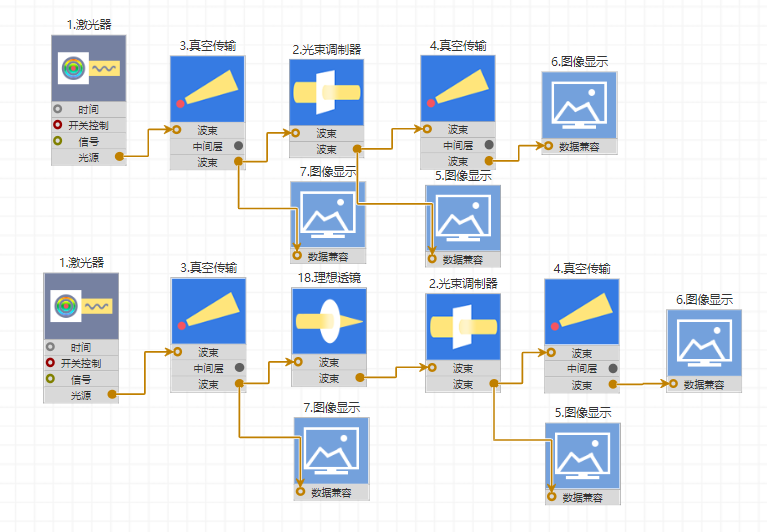
\includegraphics{img//2_2.png}
		\caption{激光的菲涅尔衍射实验}
	\end{figure}

%% 两幅图并行排版,各有图题,还有一个总的图题
	% (1)注意正文中引用图片的方法,label可以打在minipage前面,也可以打在总图题的后面。
	% (2)需要调节图片大小,也可以调节位置。通过{minipage}后面的补充参数来调节位置。图片大小可以用高度来调以保证两个图高度一样。
	\begin{figure}[htbp]
		\centering
		\subfigure[不加$\lambda/4$波片]{\label{fig:nogamma4}
		\begin{minipage}[t]{0.5\linewidth}%调节这里的图片位置
		\centering
		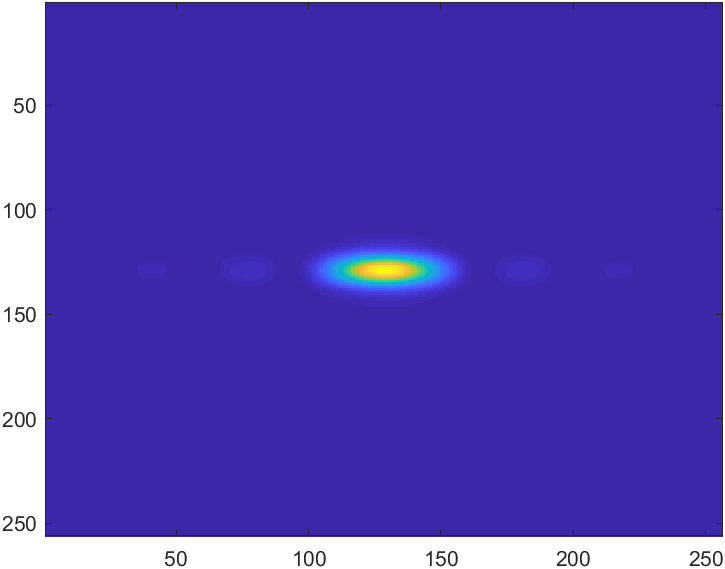
\includegraphics[width=0.8\textwidth]{img/3_1.png}%调节这里的图片宽度
		%\caption{fig1}
		\end{minipage}%
		}%
		\subfigure[加$\lambda/4$波片]{\label{fig:withgamma4}
		\begin{minipage}[t]{0.5\linewidth}%调节这里的图片位置
		\centering
		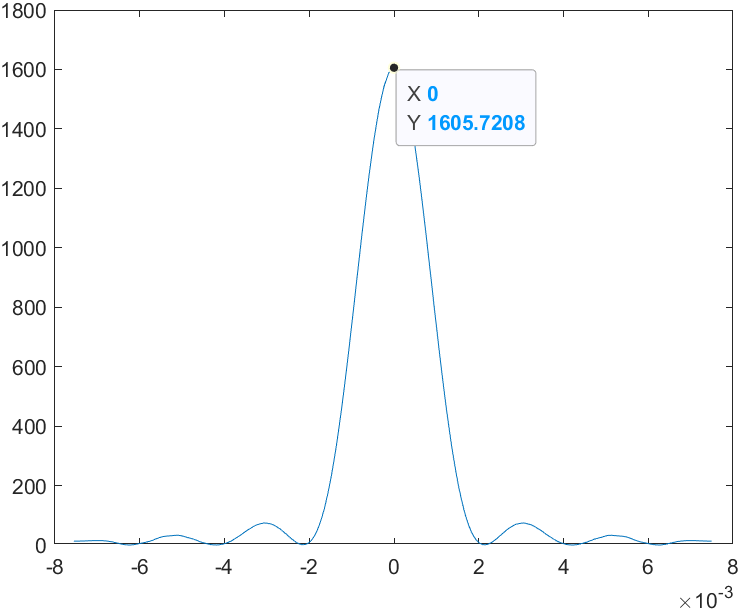
\includegraphics[width=0.8\textwidth]{img/3_2.png}%调节这里的图片宽度
		%\caption{fig2}
		\end{minipage}%
		}%
		\centering
		\caption{泡克耳斯盒的调制特性}
		\label{fig:tcvi}
	\end{figure}

%% 两幅图竖向排版,各有图题,还有一个总的图题
	% 和横向并行排版相比,关键是在两个subfigure之间空了一行!
	\begin{figure}
		\centering
		\subfigure[纵向调制]{
		\begin{minipage}[b]{0.5\textwidth}%调节这里的图片位置
			\centering
			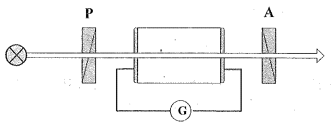
\includegraphics[width=1\textwidth]{img/v.png}%调节这里的图片宽度
		\end{minipage}
		}

		\subfigure[横向调制]{
		\begin{minipage}[b]{0.5\textwidth}%调节这里的图片位置
			\centering
			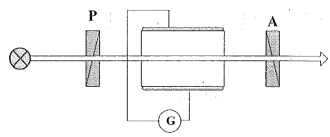
\includegraphics[width=1\textwidth]{img/h.png}%调节这里的图片宽度
		\end{minipage}
		}
		\caption{泡克尔斯盒} \label{fig:pkkeorsihe}
	\end{figure}

%% 三幅图并行排版, 各有图题, 没有总图题
	%重点:关键是给三幅图设定宽度,比如说如果希望三幅图占据等量的宽度,就可以调整每个minipage的宽度为0.3的\textwidth
	\begin{figure}[htbp]
	\centering
	\begin{minipage}{0.3\textwidth}
	\centering
			
\includegraphics[height=5cm]{img//1.eps}
			\caption{交流电桥平衡条件}
	\end{minipage}
	\hfill
	\begin{minipage}{0.3\textwidth}
	\centering
			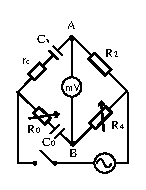
\includegraphics[height=5cm]{img//2.eps}
			\caption{电容电桥}
	\end{minipage}
	\hfill
	\begin{minipage}{0.3\textwidth}
	\centering
			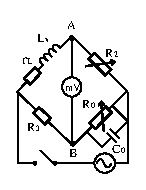
\includegraphics[height=5cm]{img//3.eps}
			\caption{麦克斯威尔-维恩电桥}
	\end{minipage}
	\end{figure}

%%%%%%%%%%%%%%%%%%%%%%%%%%%%%%%%%%%%%%%
%%%%%%%%%%%%%%%插入公式%%%%%%%%%%%%%%%%%
%%%%%%%%%%%%%%%%%%%%%%%%%%%%%%%%%%%%%%%
\newpage
	1 需要标号、单个公式
		%一般来说都需要标号
		\begin{equation}
		\eta^{\prime}=\eta /[1+b /(p a)]
		\end{equation}

	2 需要标号、多个公式、不需要对齐
		\begin{gather}
		f_r=6\pi a \eta v_g   \\
		m=4 \pi a^{3} \rho / 3
		\end{gather}

	3 需要标号、多个公式、需要对齐
		\begin{align}
		a &= b+c+d \\
		x &= y+z
		\end{align}

	4 不需要标号,单个公式
		\[e=(1.60217733 \pm 0.00000049) \times 10^{-19} \mathrm{C}\]
		另一种方法:
		\begin{equation*}
		e=(1.60217733 \pm 0.00000049) \times 10^{-19} \mathrm{C}
		\end{equation*}

	5 不需要标号,多个公式,不需要对齐/需要对齐
		%使用对应的*版本
		\begin{gather*}
		f_r=6\pi a \eta v_g   \\
		m=4 \pi a^{3} \rho / 3
		\end{gather*}
		另一种方法:
		\begin{align*}
		a &= b+c+d \\
		x &= y+z
		\end{align*}

	6 长公式,换行,不对齐
		%不标号的话加上*
		\begin{multline}
		x = a+b+c+{} \\
		d+e+f+g
		\end{multline}

	7 长公式,换行,对齐
		%aligned:次环境
		\[\begin{aligned}
		x ={}&a+b+c+{} \\
		&d+e+f+g
		\end{aligned}\]

	8 带有左边大括号的公式
	\[\left\{
		\begin{aligned}
		&C_{1} \cdot \frac{d U_{C_{1}}}{d t}=\frac{1}{R_{1}} \cdot(u_{C_{2}}-u_{C_{1}})-f(u_{R_{N}}) \\
		&C_{2} \cdot \frac{d U_{C_{2}}}{d t}=i_{L}-\frac{1}{R_{1}} \cdot(u_{C_{2}}-u_{C_{1}}) \\
		&L \cdot \frac{d i_{L}}{d t}=-U_{C_{2}}
		\end{aligned}
	   \right.
	\]


\subsection*{【思考题】}

	\subsubsection*{1.样品导热系数的大小和温度有什么关系?}
	答:关系如下:
	\begin{enumerate}[(1)]
			\item 一般固体样品导热系数与温度成线性变化,关系式为$\lambda=\lambda_0(1+\alpha t)$。$\lambda_0$是0$^{\circ}$C时固体样品的导热系数,也就是说,温度升高,导热系数变大。
			\item 少数固体和气体液体也遵循温度越高,系数越大,但呈非线性关系。
	\end{enumerate}

	\subsubsection*{2. 样品导热系数的大小与导热性能有什么关系?}
	答:导热系数的定义————在稳定传热条件下,单位温度梯度下单位时间内由单位面积传递单位厚度的热量。从以上定义可以看出,导热系数越大,反映了在材料内部传热越快,即材料本身的导热性能越好。


\newpage %换页
\subsection*{附:MATLAB中导入mat文件数据和绘制彩色强度图像和相对光强分布曲线的完整代码:}

%% 代码环境使用
	\begin{lstlisting}
	load('C:\Users\Administrator\Desktop\第1次迭代.mat')
	Intensity = Mod.^2;
	imagesc(Intensity);axis equal;
	[M,~] = size(Intensity);
	I_X = Intensity(M/2,:);
	X =-M/2:1:M/2-1;
	X = X.*ScaleATM;
	plot(X,I_X);
	\end{lstlisting}


\end{document}
